\documentclass[a4paper, 12pt]{article}
\usepackage[utf8]{inputenc}
\usepackage[english,russian]{babel}
\usepackage[warn]{mathtext}
\usepackage{graphicx}
\usepackage{float}
\usepackage{multirow}
\restylefloat{table}
\usepackage{amsmath}
\usepackage{floatflt}
\usepackage[T2A]{fontenc}
\usepackage[left=20mm, top=20mm, right=20mm, bottom=20mm, footskip=10mm]{geometry}
\usepackage{amssymb}

\tolerance 1414
\hbadness 1414
\emergencystretch 1.5em
\hfuzz 0.3pt        % размер максимального переполнения без warning'a
\widowpenalty=10000 % запрещает одиночную строку абзаца в начале страницы
\vfuzz \hfuzz
\raggedbottom       % если на странице мало содержимого, добавить пустое место в конце, а не в середине страницы



\begin{document}

\begin{titlepage}
	\centering
	\vspace{5cm}
	{\scshape\LARGE московский физико-технический институт (национальный исследовательский университет) \par}
	\vspace{6cm}
	{\scshape\Large Лабораторная работа 4.3.6 \par}
	{\huge\bfseries Саморепродукция \par}
	\vspace{1cm}
	\vfill
\begin{flushright}
	{\large Б03-102}\par
	\vspace{0.3cm}
	{\LARGE Куланов Александр}
\end{flushright}
	

	\vfill


	Долгопрудный, 2023 г.
\end{titlepage}

\begin{itemize}
	\item \textbf{Цель работы:} изучение явления саморепродукции и применение его к измерению параметров периодических структур
    \item \textbf{В работе используются:} лазер, кассета с сетками, мира, короткофокусная линза с микрометрическим винтом, экран, линейка
\end{itemize}

\section{Экспериментальная установка}

\begin{figure}[H]
    \centering
    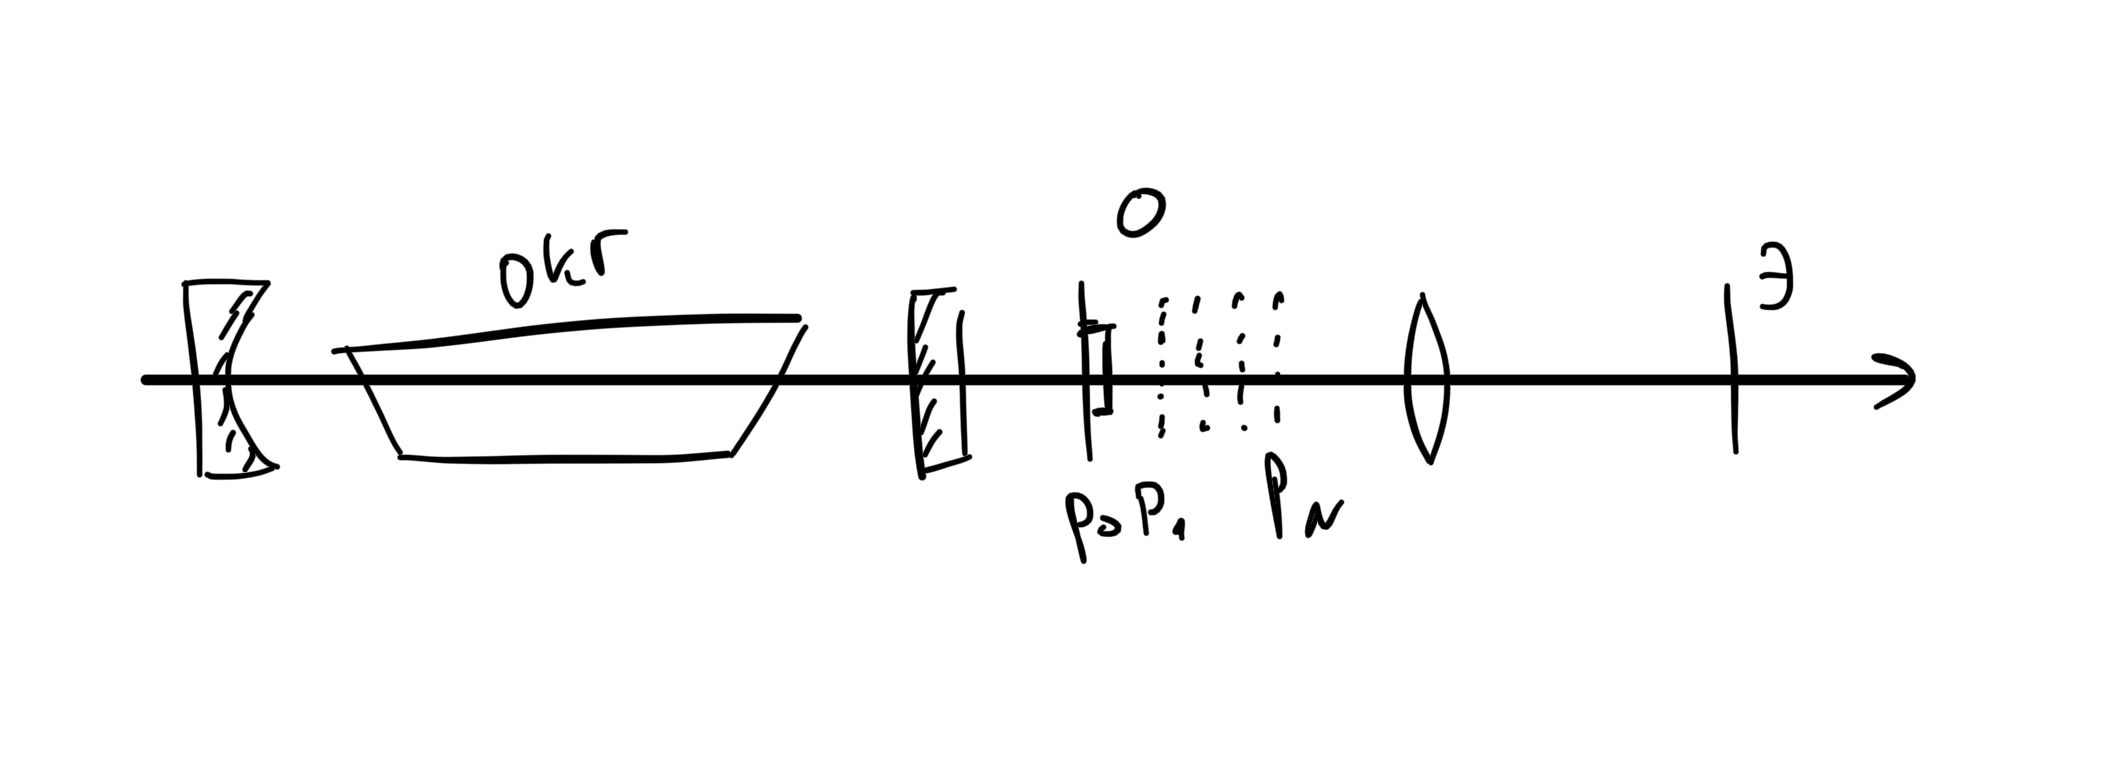
\includegraphics[width=1\textwidth]{set.jpg}
    \caption{Экспериментальная установка}
    \label{fig:set}
\end{figure}

ОКГ --- гелий-неоновый лазер, 0 --- двумерная решетка, PN --- плоскости, где наблюдаются репродуцированные изображения, Л --- короткофокусная линза, Э --- экран для наблюдения изображения объекта

За плоскостью P0 периодически по z возникают изображения объекта, которые с помощью линзы Л можно поочередно проецировать на экран, установленный в плоскости Э.
Если убрать линзу, то на экране наблюдается картина дифракции луча на периодическом объекте.

Экран устанавливается достаточно далеко от объекта, так что продифрагированные лучи, соответствующие различным порядкам дифракции, разделяются.

Измерив расстояние от объекта до экрана, можно определить $\sin \varphi$ и $d$


\section{Ход работы и обработка результатов}

В работе сделаем следующее:
\begin{itemize}
	\item определим периоды сеток сначала по их спектру на экране, потом по увеличенному изображению, затем по расстоянием между репродуцированными изображениями
	\item то же самое для элементов миры 
\end{itemize}

\subsection{Исследование двумерных решеток}
\subsubsection*{Определение периода решеток по их пространственному спектру}

Поставим перед лазером кассету с двумерными решетками. На экране увидим дифракционную картину. Определим расстояние между соседними максимумами.

\begin{table}[H]
	\centering
	\begin{tabular}{|c|c|c|c|}
	\hline
	\textbf{Сетка, №} & \textbf{l, мм} & \textbf{m} & \textbf{x, мм} \\ \hline
	1                 & 36,5           & 1          & 36,5           \\ \hline
	2                 & 50             & 2          & 25,0           \\ \hline
	3                 & 85             & 7          & 12,1           \\ \hline
	4                 & 50             & 9          & 5,6            \\ \hline
	5                 & 60             & 13         & 4,6            \\ \hline
	\end{tabular}
	\caption{Данные}
	\label{tab:data1}
\end{table}
Период решеток можем вычислить по формуле:

\begin{equation}
	d = \frac{m \lambda}{\sin \varphi} \approx \frac{\lambda L}{x}
\end{equation}
где L - расстояние между решеткой и экраном, равное 1349 мм в нашем случае. Длина волны лазера 510 нм.

\begin{table}[H]
	\centering
	\begin{tabular}{|c|c|}
	\hline
	\textbf{Сетка, №} & \textbf{d, мм} \\ \hline
	1                 & 0,019         \\ \hline
	2                 & 0,028         \\ \hline
	3                 & 0,057         \\ \hline
	4                 & 0,124         \\ \hline
	5                 & 0,149         \\ \hline
	\end{tabular}
	\caption{Периоды решеток}
	\label{tab:res1}
\end{table}

\subsubsection*{Определение периода решёток по изображению, увеличенному с помощью линзы}

Закрепим короткофокусную линзу на небольшом расстоянии от лазера. Уберем кассету и центрируем систему. Затем установим кассету с сетками между лазером и линзой.
Перемещая изображение сетки вдоль оси системы, получим на экране увеличенное изображение сетки.

Наведем резкость на тонкую проволчку на одной из сеток, чтобы наблюдать геометрическое изображение, а не репродуцированное. Определим размеры D клеток на экране.
В нашем случае это возможно только для сеток с номерами 2, 3, 4 и 5.

Расстояние от линзы до экрана $b = 1294$ мм. Расстояние от линзы до сетки $a = 55$ мм.
По полученным данным рассчитаем периоды сеток по формуле:

\begin{equation}
	d = \frac{Da}{b}
\end{equation}


\begin{table}[H]
	\centering
	\begin{tabular}{|c|c|c|}
	\hline
	\textbf{Сетка, №} & \textbf{D, мм} & \textbf{d, мм} \\ \hline
	2                 & 0,5            & 0,021          \\ \hline
	3                 & 1,5            & 0,064          \\ \hline
	4                 & 3              & 0,128          \\ \hline
	5                 & 3,5            & 0,149          \\ \hline
	\end{tabular}
	\caption{Данные и результаты}
	\label{tab:data2}
	\end{table}

\subsubsection*{Исследование эффекта саморепродукции с помощью сеток}

Получим на экране геометрическое изображение сетки. Перемещая линзу с помощью микровинта, определим координаты $z_n$ плоскостей саморепродукции.

Построим графики зависимости $z_n$ от номера решетки. Из формулы 

\begin{equation}
	z_n = \frac{2d^2n}{\lambda}
\end{equation}

Выразим d через угол наклона прямой в полученных графиках:

\begin{equation}
	d = \sqrt{\frac{k\lambda}{2}}
\end{equation}

\begin{figure}[H]
    \centering
    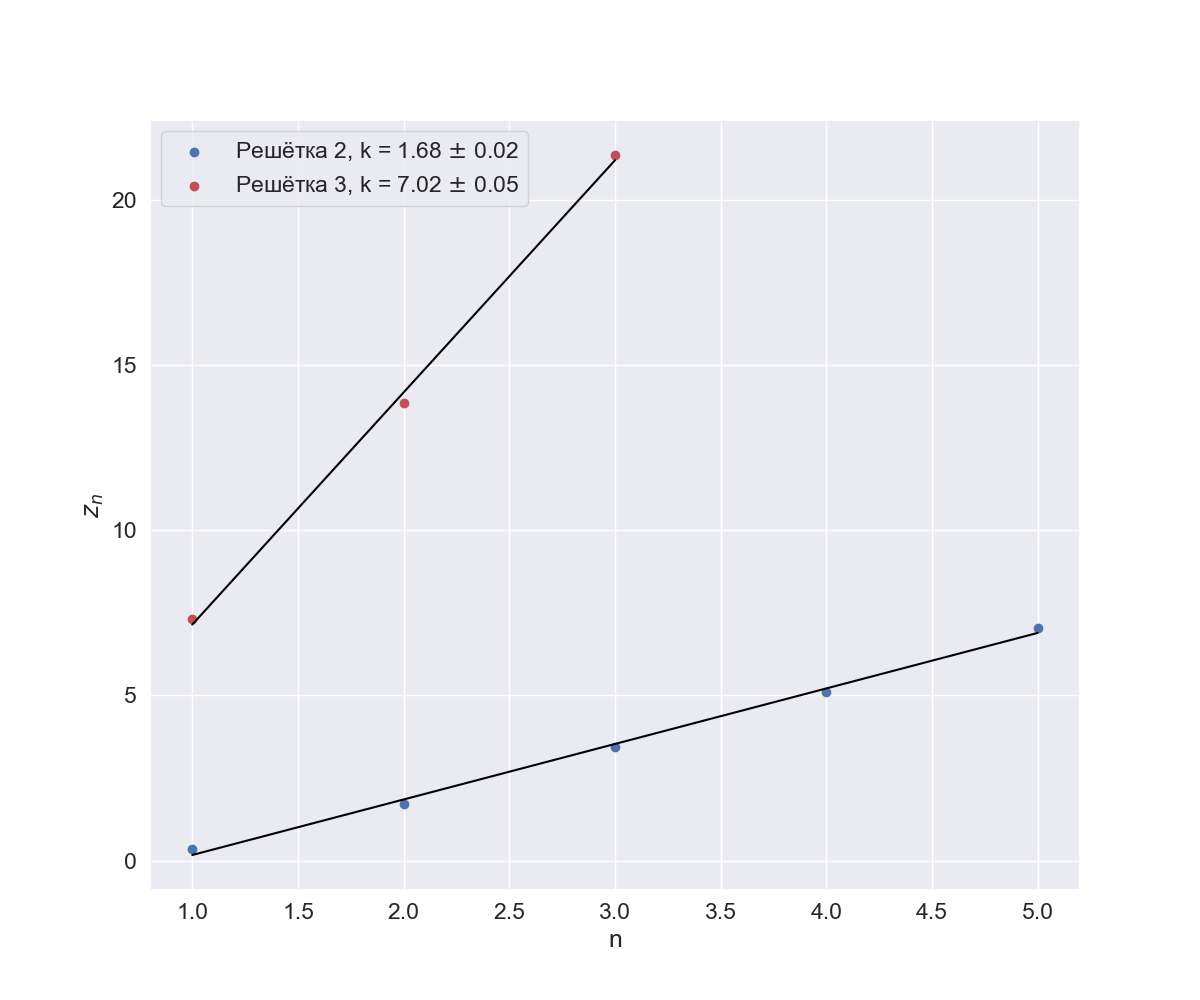
\includegraphics[width=1\textwidth]{plot1.png}
    \caption{зависимости $z_n$ от номера $n$}
    \label{fig:plo1}
\end{figure}

\begin{table}[H]
	\centering
	\begin{tabular}{|c|c|}
	\hline
	\textbf{Сетка, №} & \textbf{d, мм} \\ \hline
	2                 & 0,020           \\ \hline
	3                 & 0,042          \\ \hline
	\end{tabular}
	\caption{Результаты}
	\label{tab:res2}
	\end{table}

\subsubsection*{Выводы}

Приведем сводную таблицу по всем методам:

\begin{table}[H]
	\centering
	\begin{tabular}{|c|ccc|}
	\hline
	\textbf{}         & \multicolumn{1}{c|}{\textbf{Спектр}} & \multicolumn{1}{c|}{\textbf{Линза}} & \textbf{Саморепродукция} \\ \hline
	\textbf{Сетка, №} & \multicolumn{3}{c|}{\textbf{d, мм}}                                                                   \\ \hline
	1                 & \multicolumn{1}{c|}{0,019}           & \multicolumn{1}{c|}{}               &                          \\ \hline
	2                 & \multicolumn{1}{c|}{0,028}           & \multicolumn{1}{c|}{0,021}          & 0,020                    \\ \hline
	3                 & \multicolumn{1}{c|}{0,057}           & \multicolumn{1}{c|}{0,064}          & 0,042                    \\ \hline
	4                 & \multicolumn{1}{c|}{0,124}           & \multicolumn{1}{c|}{0,128}          &                          \\ \hline
	5                 & \multicolumn{1}{c|}{0,149}           & \multicolumn{1}{c|}{0,149}          &                          \\ \hline
	\end{tabular}
	\caption{Сводная таблица}
	\label{tab:res}
	\end{table}

Как можно видеть, первые два способа дают сопоставимые результаты. Третий способ дает немного другие результаты, так как во время выполнения было тяжело визуально наблюдать саморепродукцию. Для некоторых решеток и вовсе не получилось собрать данные.
Так же следует сказать, что большую погрешность в результаты внесло определение расстояние до экрана, так как не было линейки подходящей длины.

\subsection{Исследование миры}

Поставим миру на место решетки в предыдущем пункте. Исследуем саморепродукцию изображения одного из элеметнов миры:


\begin{figure}[H]
	\centering
	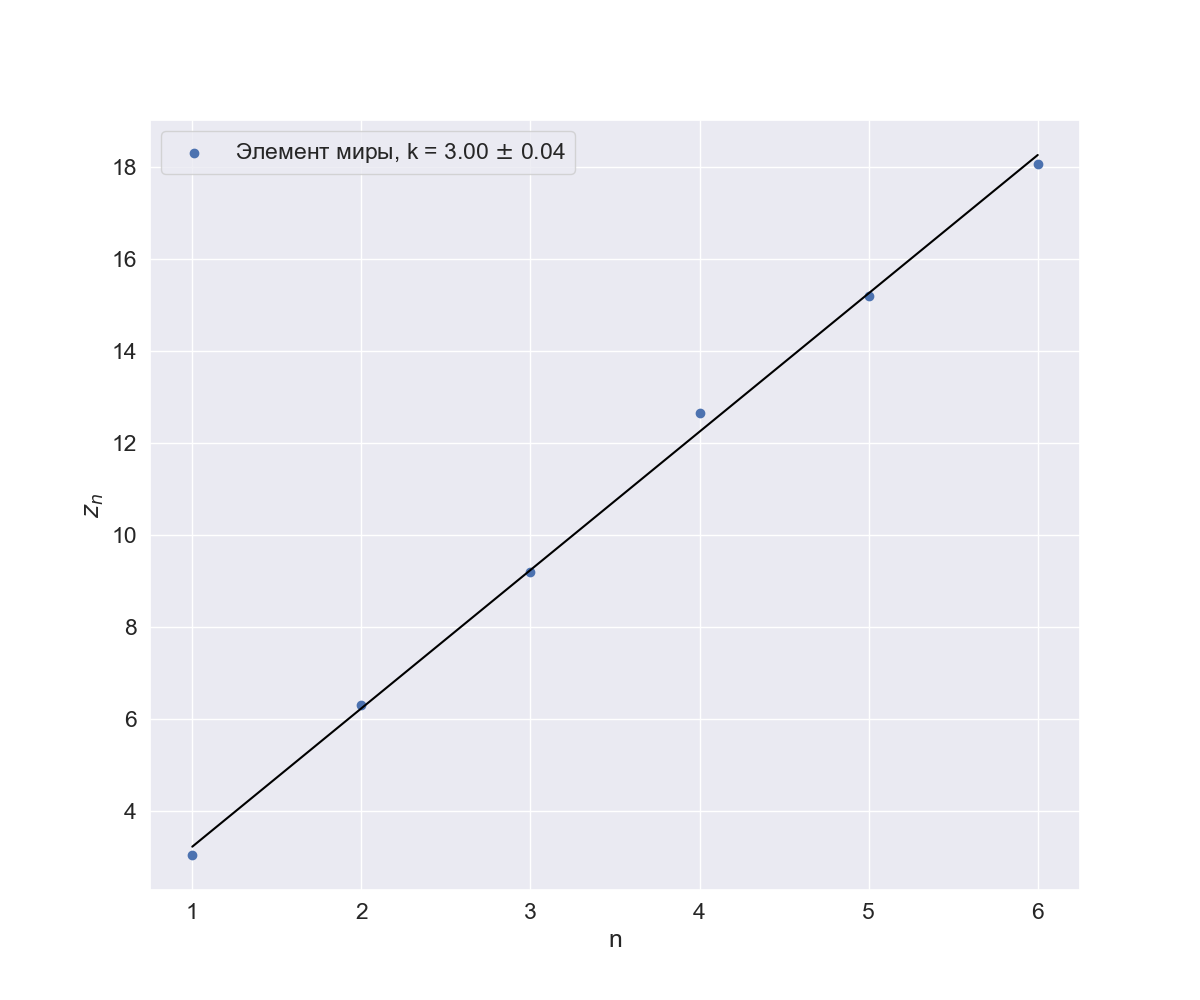
\includegraphics[width=0.8\textwidth]{plot2.png}
	\caption{зависимости $z_n$ от номера $n$}
	\label{fig:plo2}
\end{figure}

\begin{table}[H]
	\centering
	\begin{tabular}{|c|c|}
	\hline
	\textbf{$n$} & \textbf{$z_n$, мм} \\ \hline
	1              & 3,05           \\ \hline
	2              & 6,3            \\ \hline
	3              & 9,2            \\ \hline
	4              & 12,65          \\ \hline
	5              & 15,2           \\ \hline
	6              & 18,05          \\ \hline
	\end{tabular}
	\caption{Данные}
	\label{tab:datamir}
	\end{table}

По формуле 4 найдем d. Получилось
\begin{equation}
	\mathbf{d = 0.027 \text{ мм}}
\end{equation}

\end{document}